\documentclass[portrait,a0paper,fontscale=0.35]{baposter}

\usepackage{calc}
\usepackage{graphicx}
\usepackage{amsmath}
\usepackage{amssymb}
\usepackage{relsize}
\usepackage{multicol}
\usepackage{multirow}
\usepackage{rotating}
\usepackage{bm}
\usepackage{url}
\usepackage{color}

\usepackage{graphicx}
\usepackage{multicol}

\begin{document}

\begin{poster}{
  grid=false,
  columns=4,
  colspacing=1em,
  bgColorOne=white,
  bgColorTwo=white,
  borderColor=blue,
  headerColorOne=black,
  headerColorTwo=blue,
  headerFontColor=white,
  boxColorOne=white,
  boxColorTwo=blue,
  textborder=roundedleft,
  eyecatcher=true,
  headerborder=closed,
  headerheight=0.1\textheight,
  headershape=roundedright,
  headershade=shadelr,
  headerfont=\Large\bf\textsc,
  textfont={\setlength{\parindent}{1.5em}},
  boxshade=plain,
  background=plain,
  linewidth=2pt
  }
  {
  }
  {\bf\textsc{Analysis of the Biomodels Database}\vspace{0.5em}}
  {Unknown Author}
  {
  }
  
 \headerbox{Biomodels Database}{name=biomodelsdatabase,column=0,row=0}{
 Biomodels Database is an online resource for storing and serving quantative models of biomedical  interest. The datbase was created in 2005. 
 
 The focus of the project is the curated branch of the database. There are currently 424 models in this branch. These models have been described in peer reviewed sceintific literature.
 
 One of the programming languages used by modellers submitting to the biomodels datbase is SBML. The models can also be downloaded from the database in SBML format.
 
 }
  
  \headerbox{R}{name=r, column=1,row=0}{
  R is a computer package that is widely used for statistical software
development and data analysis. The system
provides a wide variety of statistical and graphical techniques.
 
 R is highly extensible through the use of user-submitted libraries for
specific functions or specific areas of study. An example of this is the package rsbml, which was used in order to read models into R and extract information from the models.
 
 A particular strength of R is its graphical facilities, which produce quality graphs that can include
mathematical symbols.
  }
 
 \headerbox{Species and Reactions}{name=specsnreacts,column=2,row=0,span=2}{
 \begin{multicols}{2}
 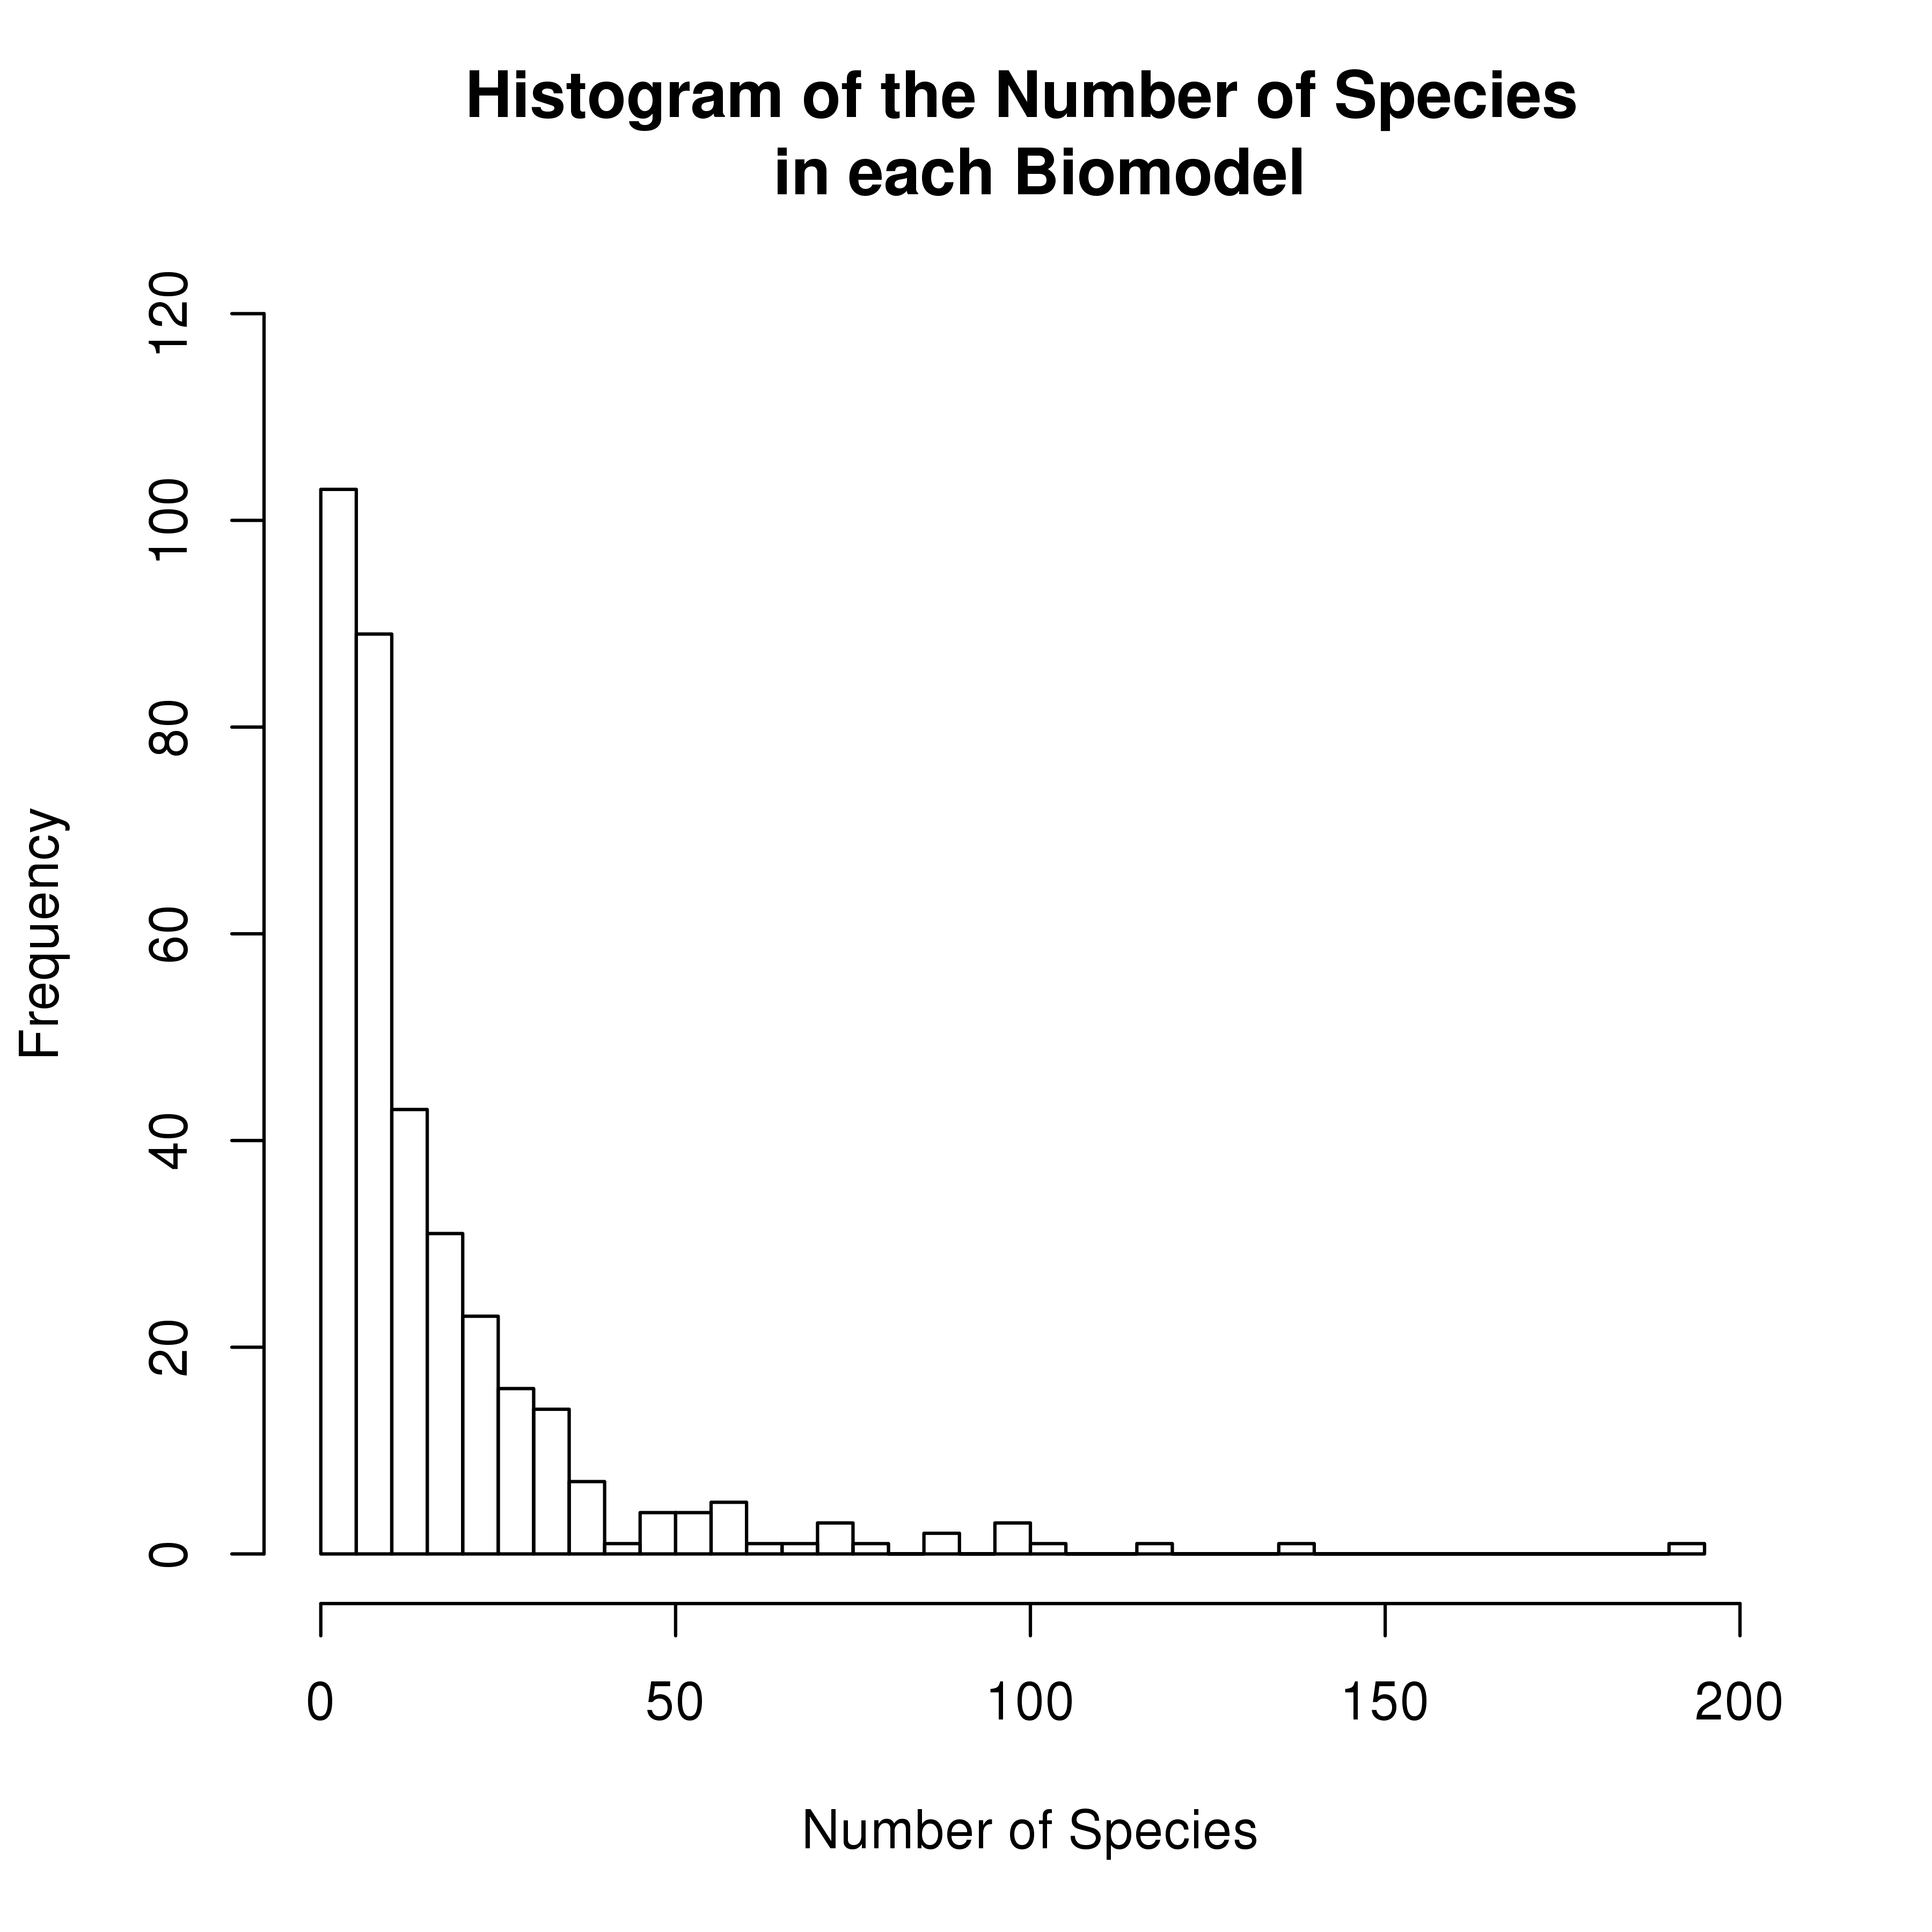
\includegraphics[trim= 1.5mm 5mm 5mm 5mm, clip, scale=0.4]{Poster-images/SpeciesHistogram.png}
 
 The grpah above is the histogram of the number of species in each biomodel. The majority of models have 10 or less species, suggesting that the models tend to have small numbers of species.\\
 
 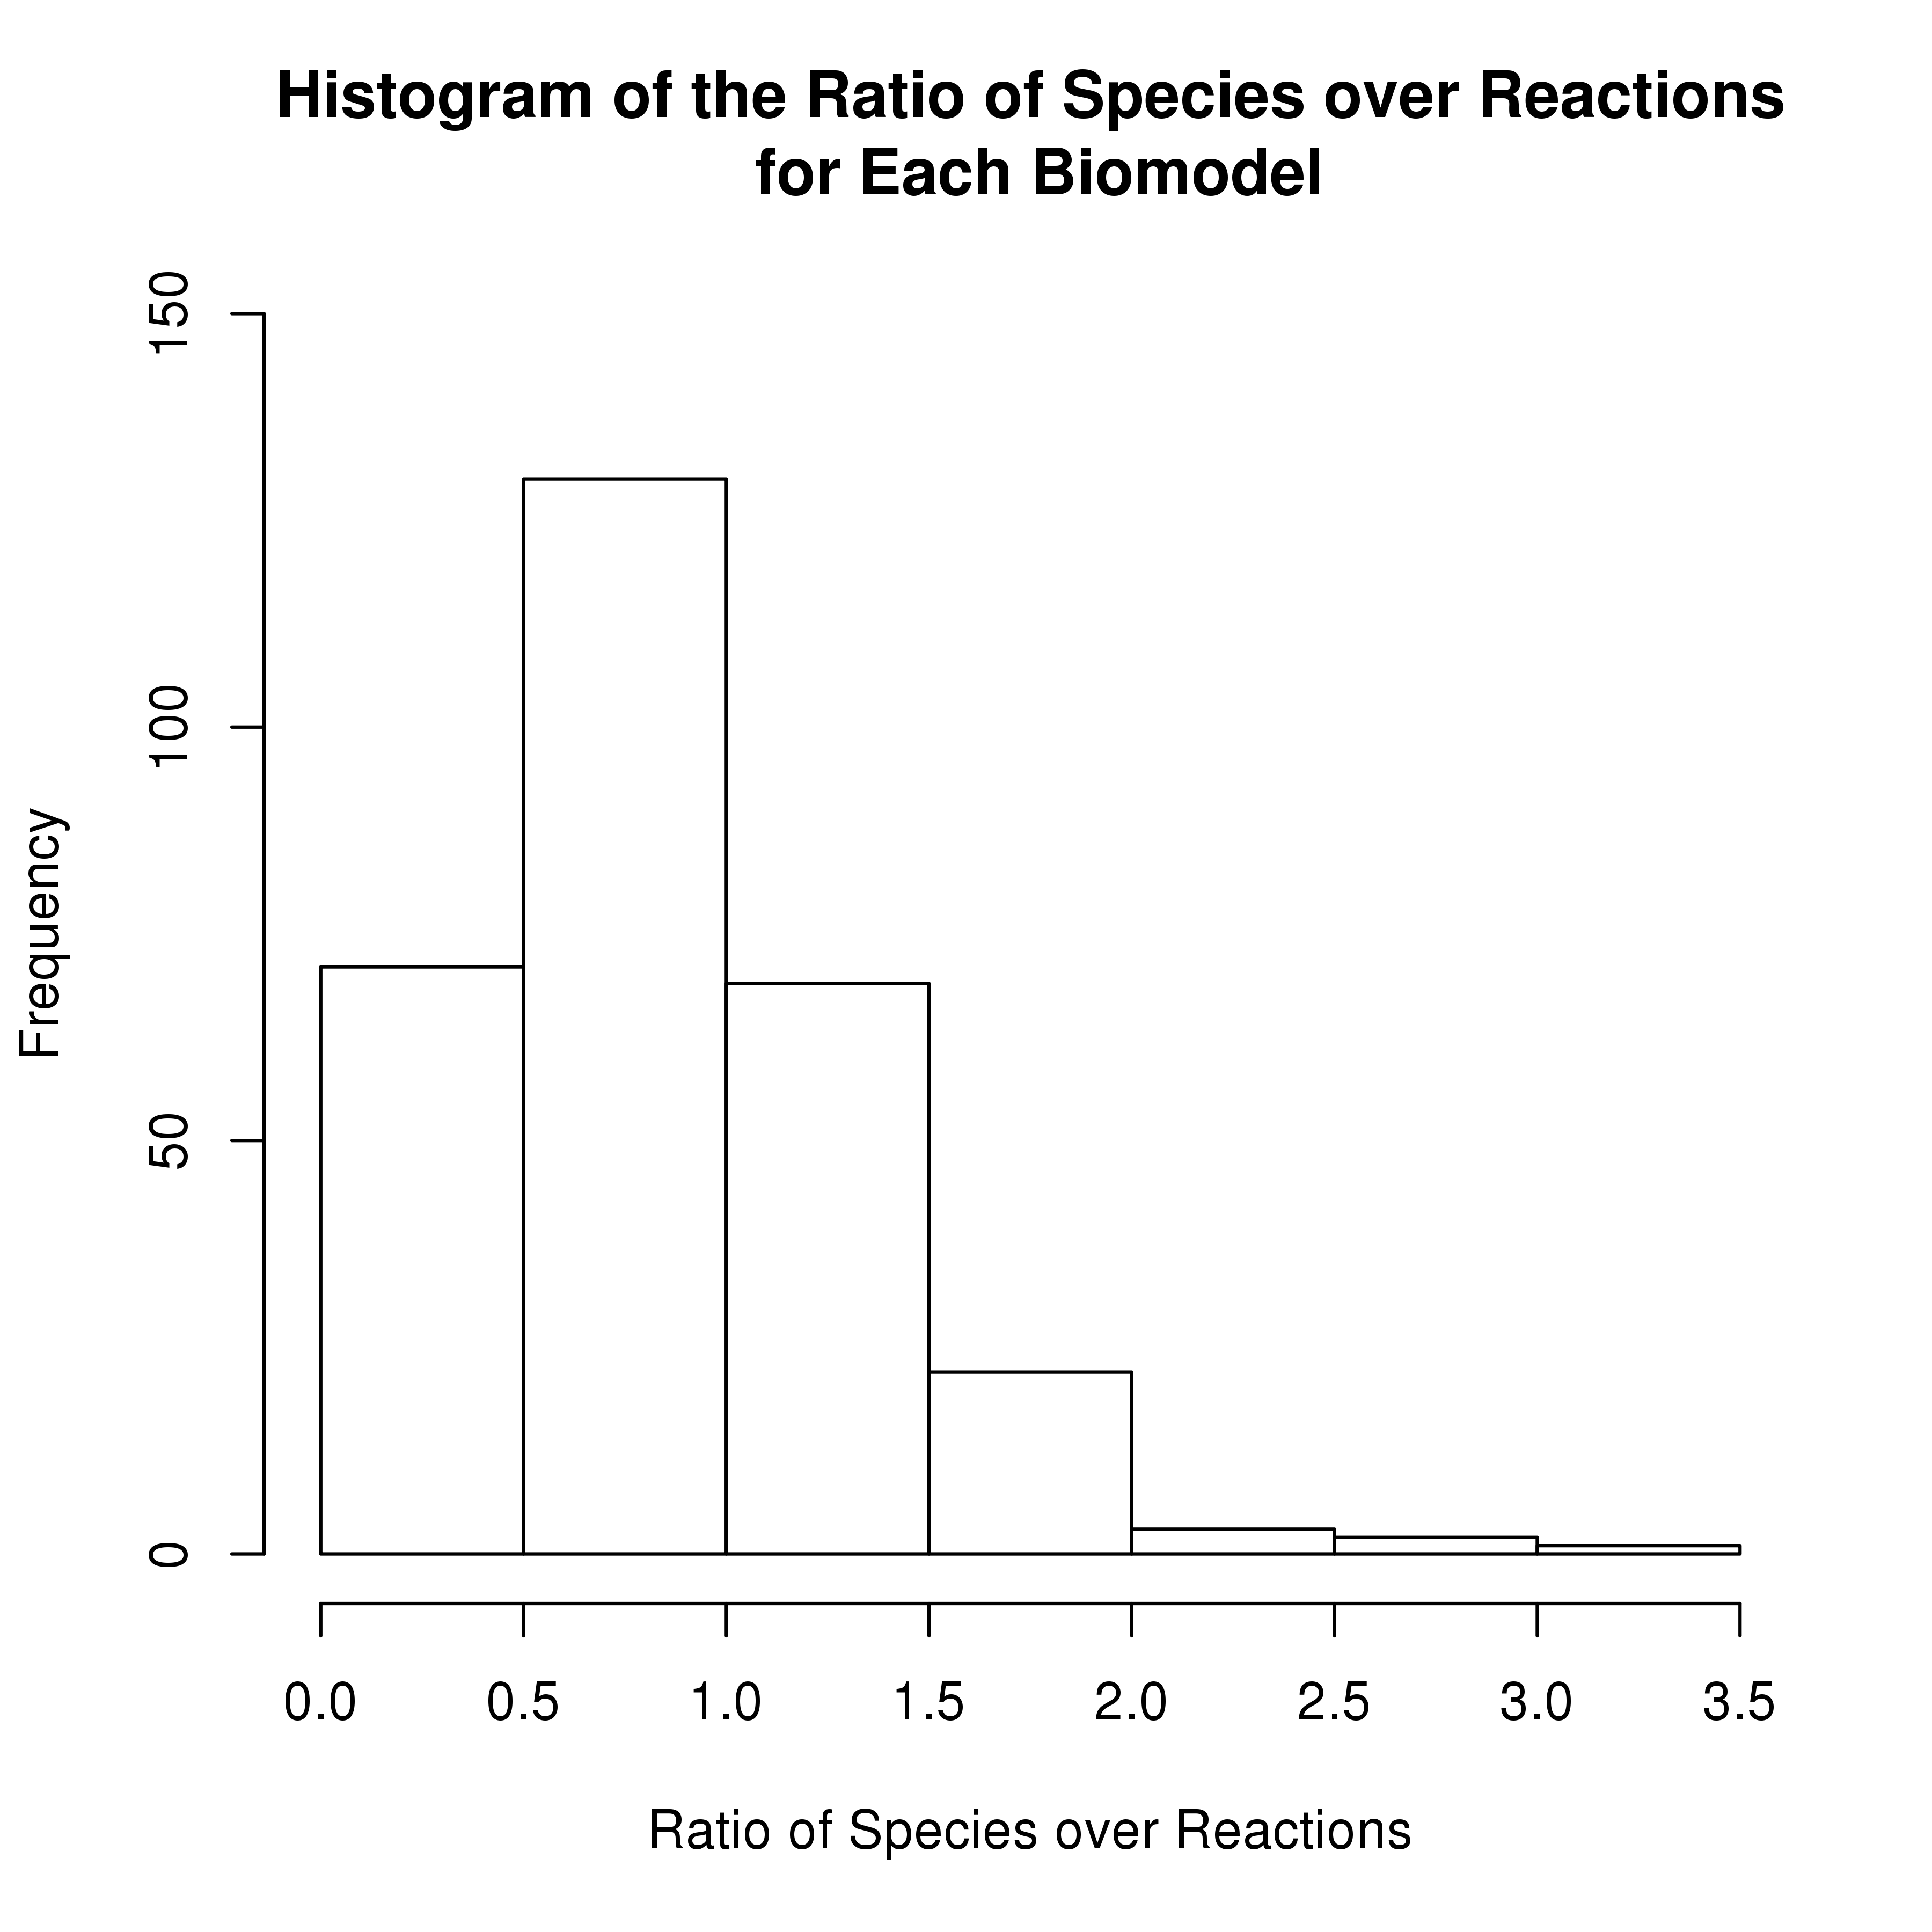
\includegraphics[trim= 1.5mm 5mm 5mm 5mm, clip, scale=0.4]{Poster-images/SpeciesOverReactions.png}
 
 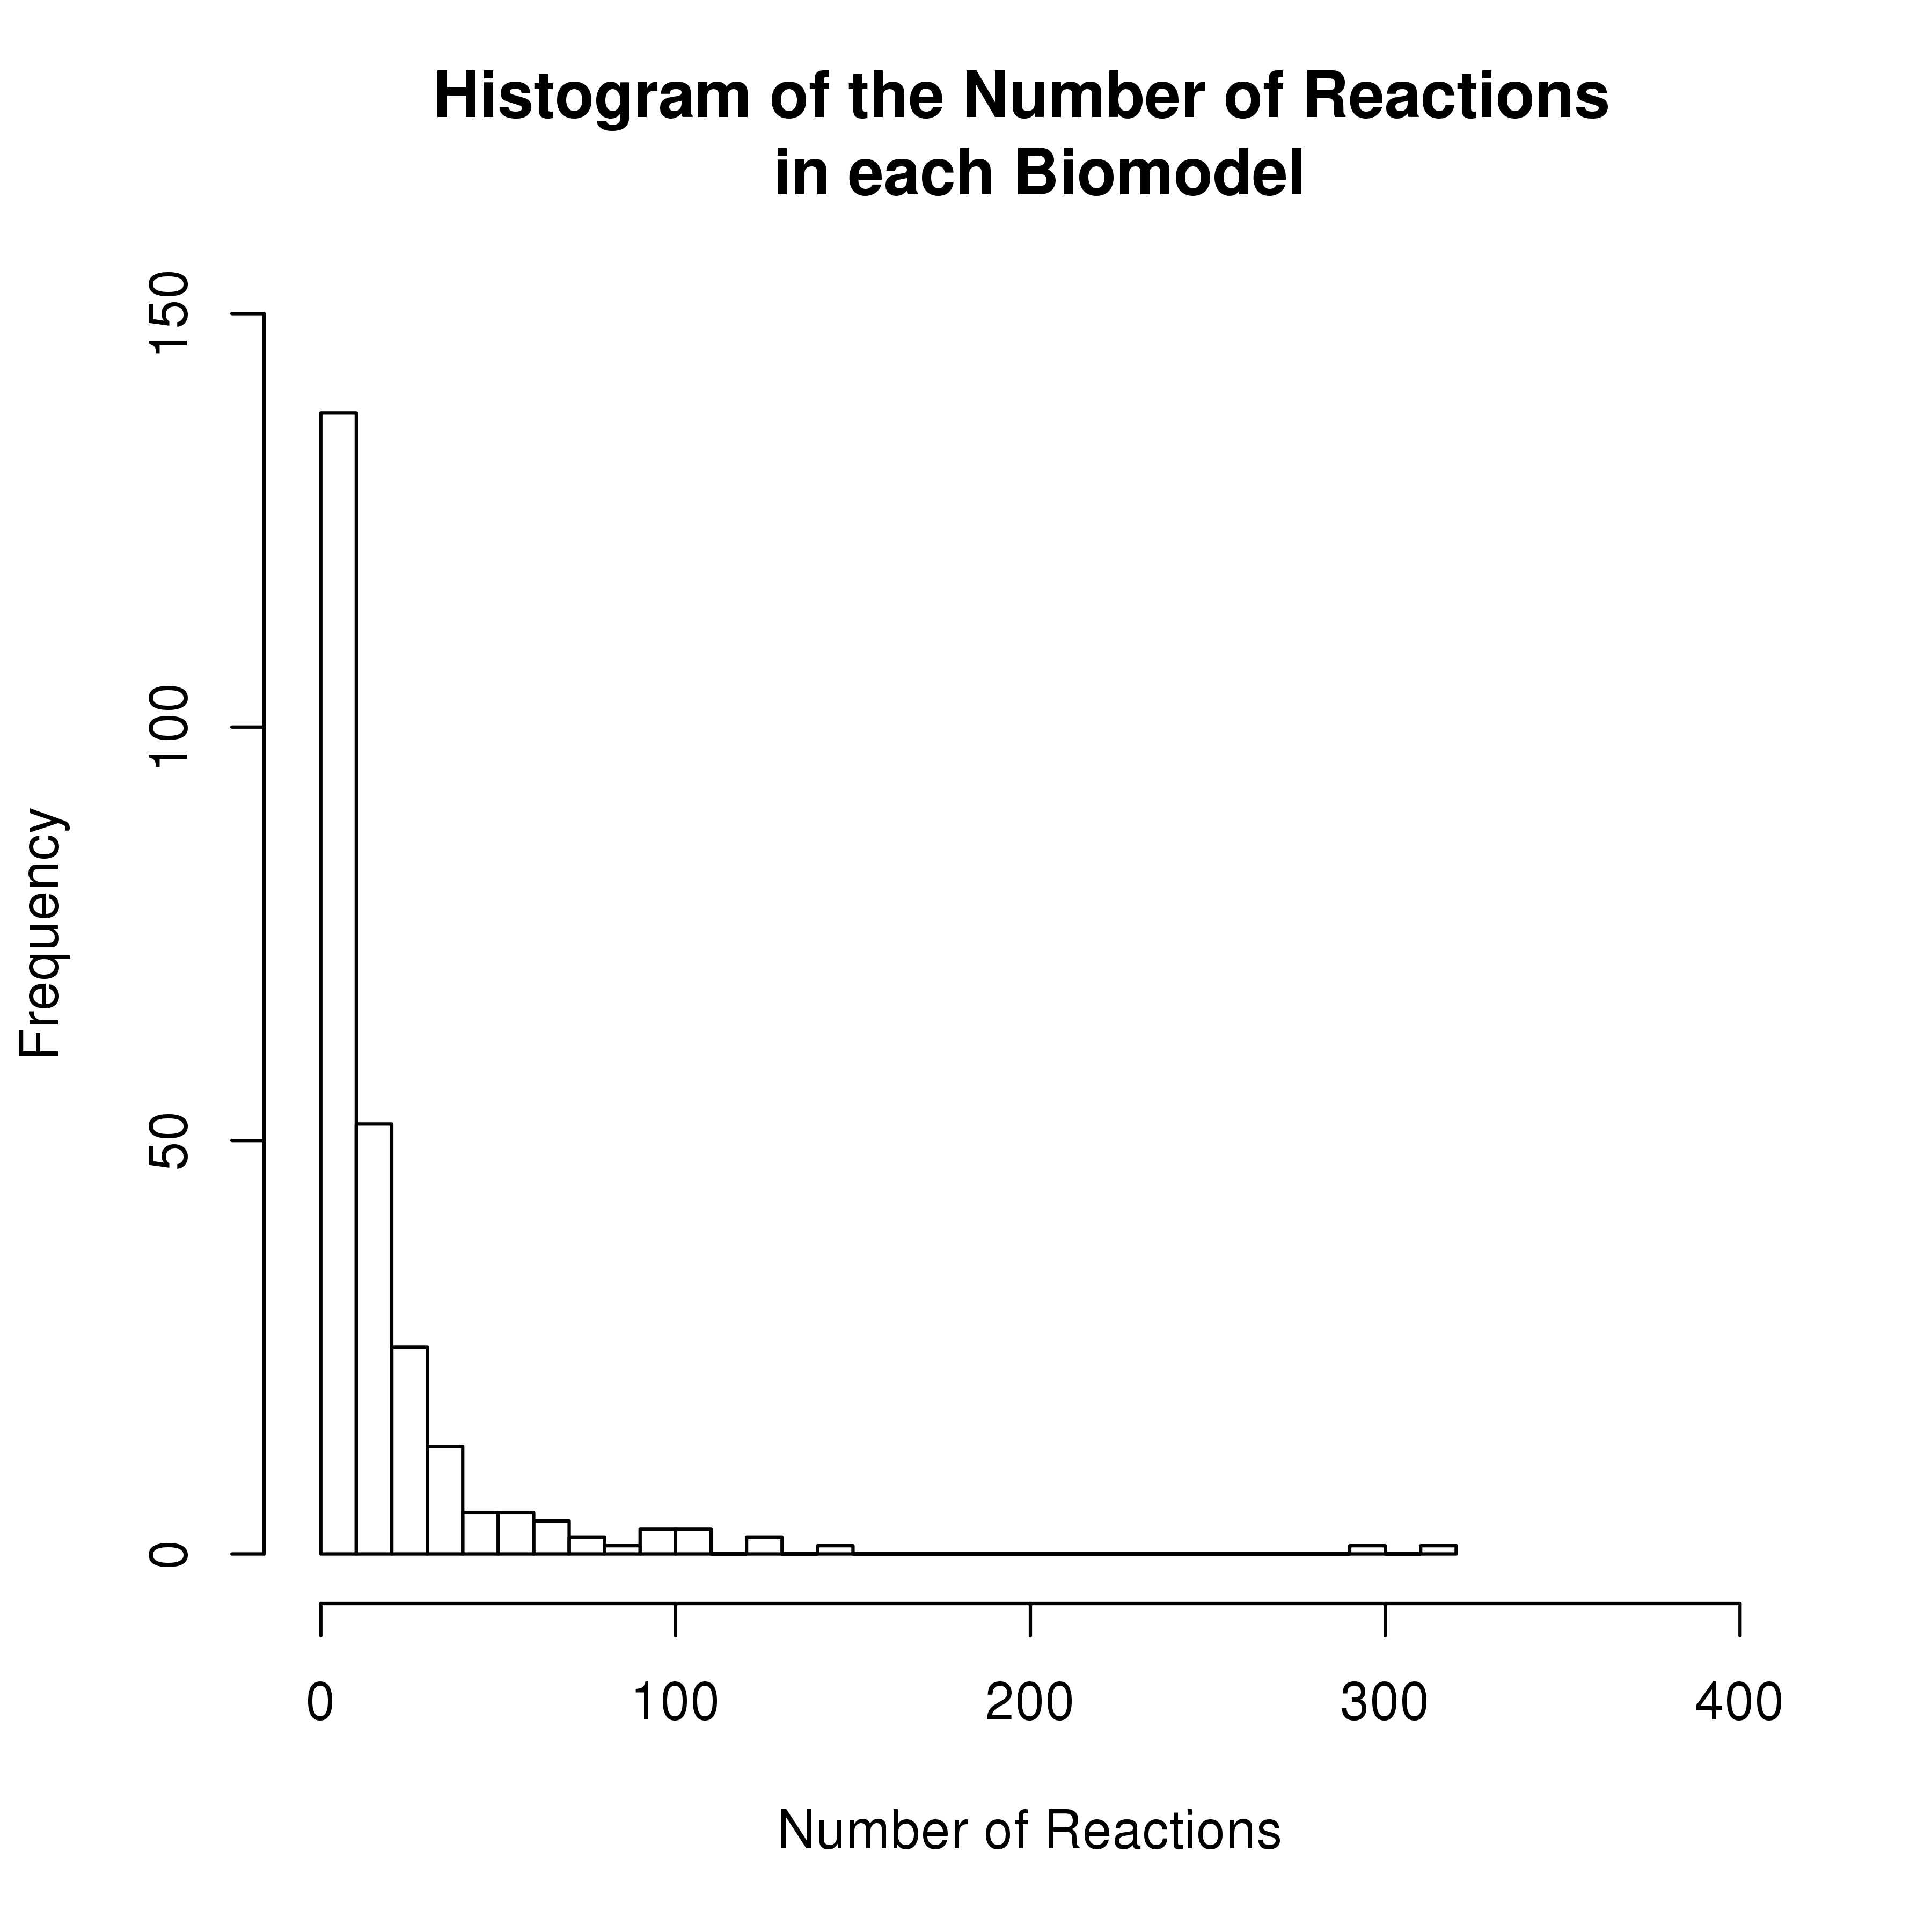
\includegraphics[trim= 1.5mm 5mm 5mm 5mm, clip, scale=0.4]{Poster-images/ReactionsHistogram.png} 
  
  The grpah above is the histogram of the number of reactions in each biomodel. The graph has a similar pattern to the species histogram, suggesting that the models tend to have low numbers of reactions.\\
   
 The graph to the left is a histogram of the ratio of species to reactions in each biomodel. The most frequent range is range of values is 0.5-1.0 with the majority of models having ratios less than 2.
 
 This suggests that in the majority of models, the species tend to appear in multiple reactions. This is because if every species in a model appeared in exactly one reaction, the ratio of species to reactions would be at least 2 as each reaction has at least one reactant and one product.
 
 \end{multicols}
 }
 
 
 \headerbox{References}{name=sboterms,column=0,above=bottom}{
 
 }
 
 \headerbox{Conlcusion}{name=conclusion,column=1,above=bottom}{
 
 }
 
 \headerbox{More Pretty Pictures}{name=moreprettypics,column=2,span=2,above=bottom}{
 \begin{multicols}{2}
 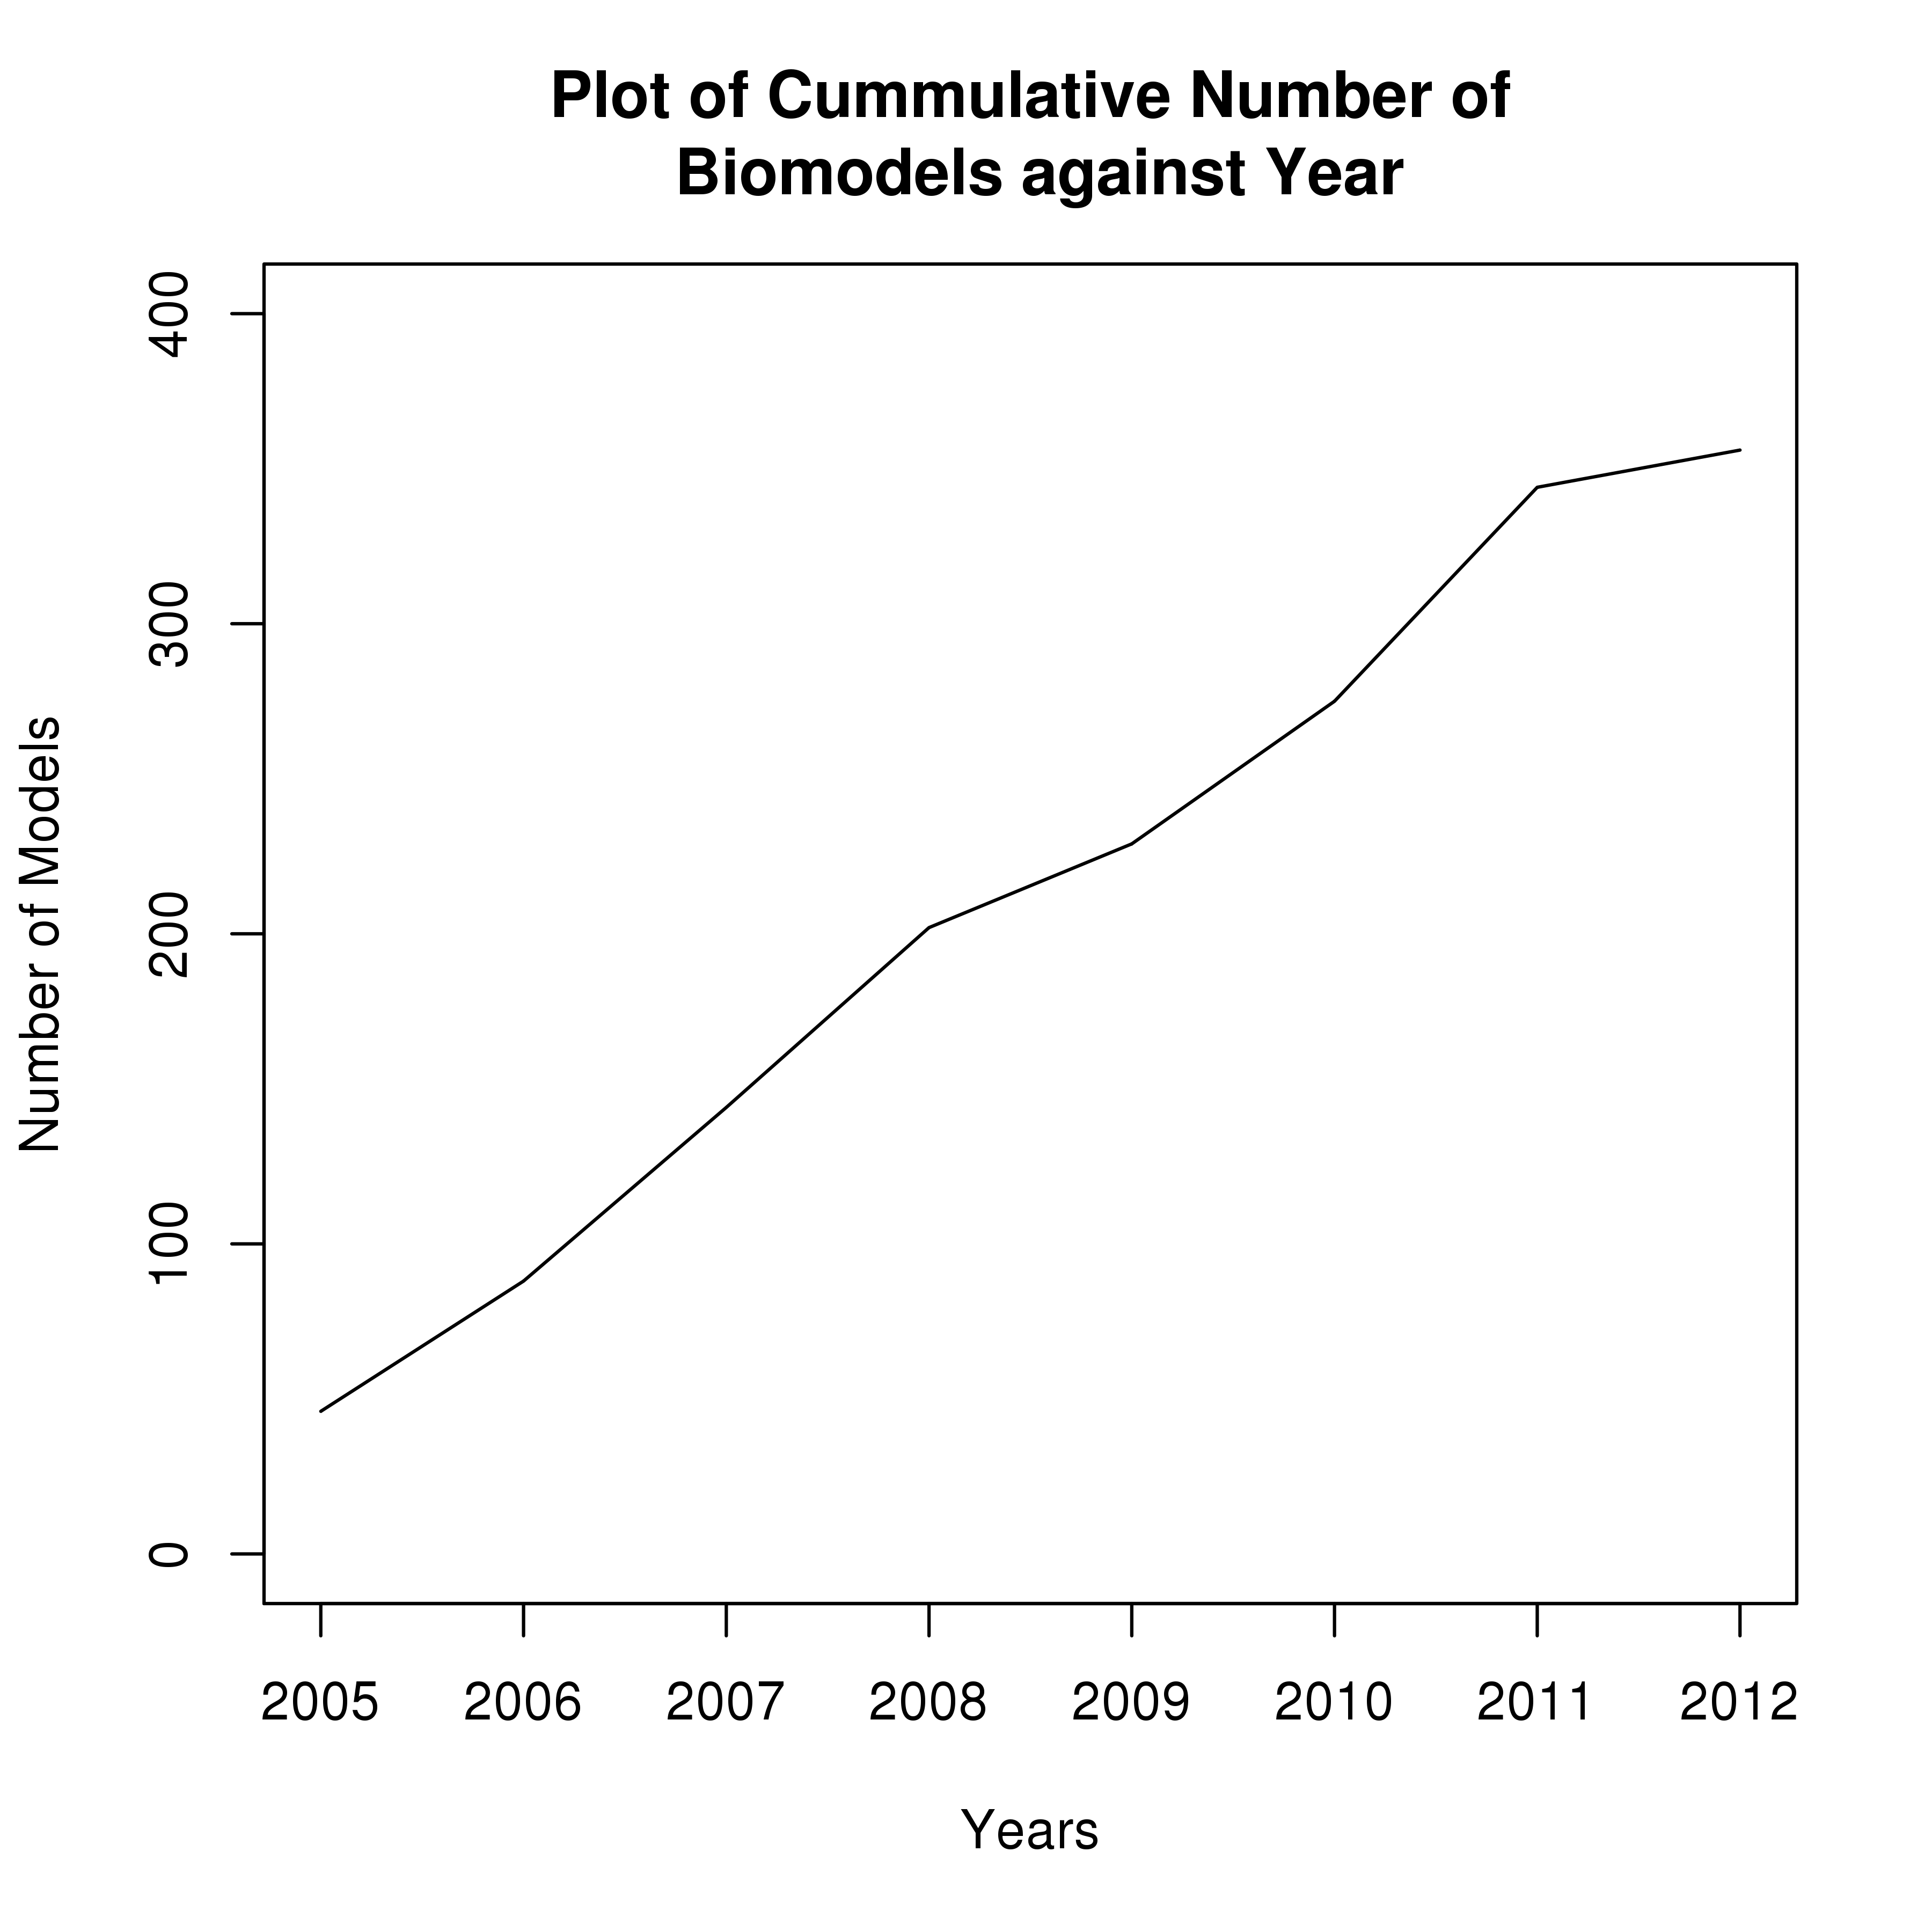
\includegraphics[trim= 1.5mm 5mm 5mm 4.5mm, clip, scale=0.4]{Poster-images/CummulativeModelsPlot.png}
 The graph above shows the number of biomodels in the curated branch against time. The increase in the number of models appears to be close to linear, suggesting the rate at which models are being added to the curated branch is reasonbly constant.

 The latest archive used in the project was the August 2012 archive, hence the small increase in 2012 is expected.
 
 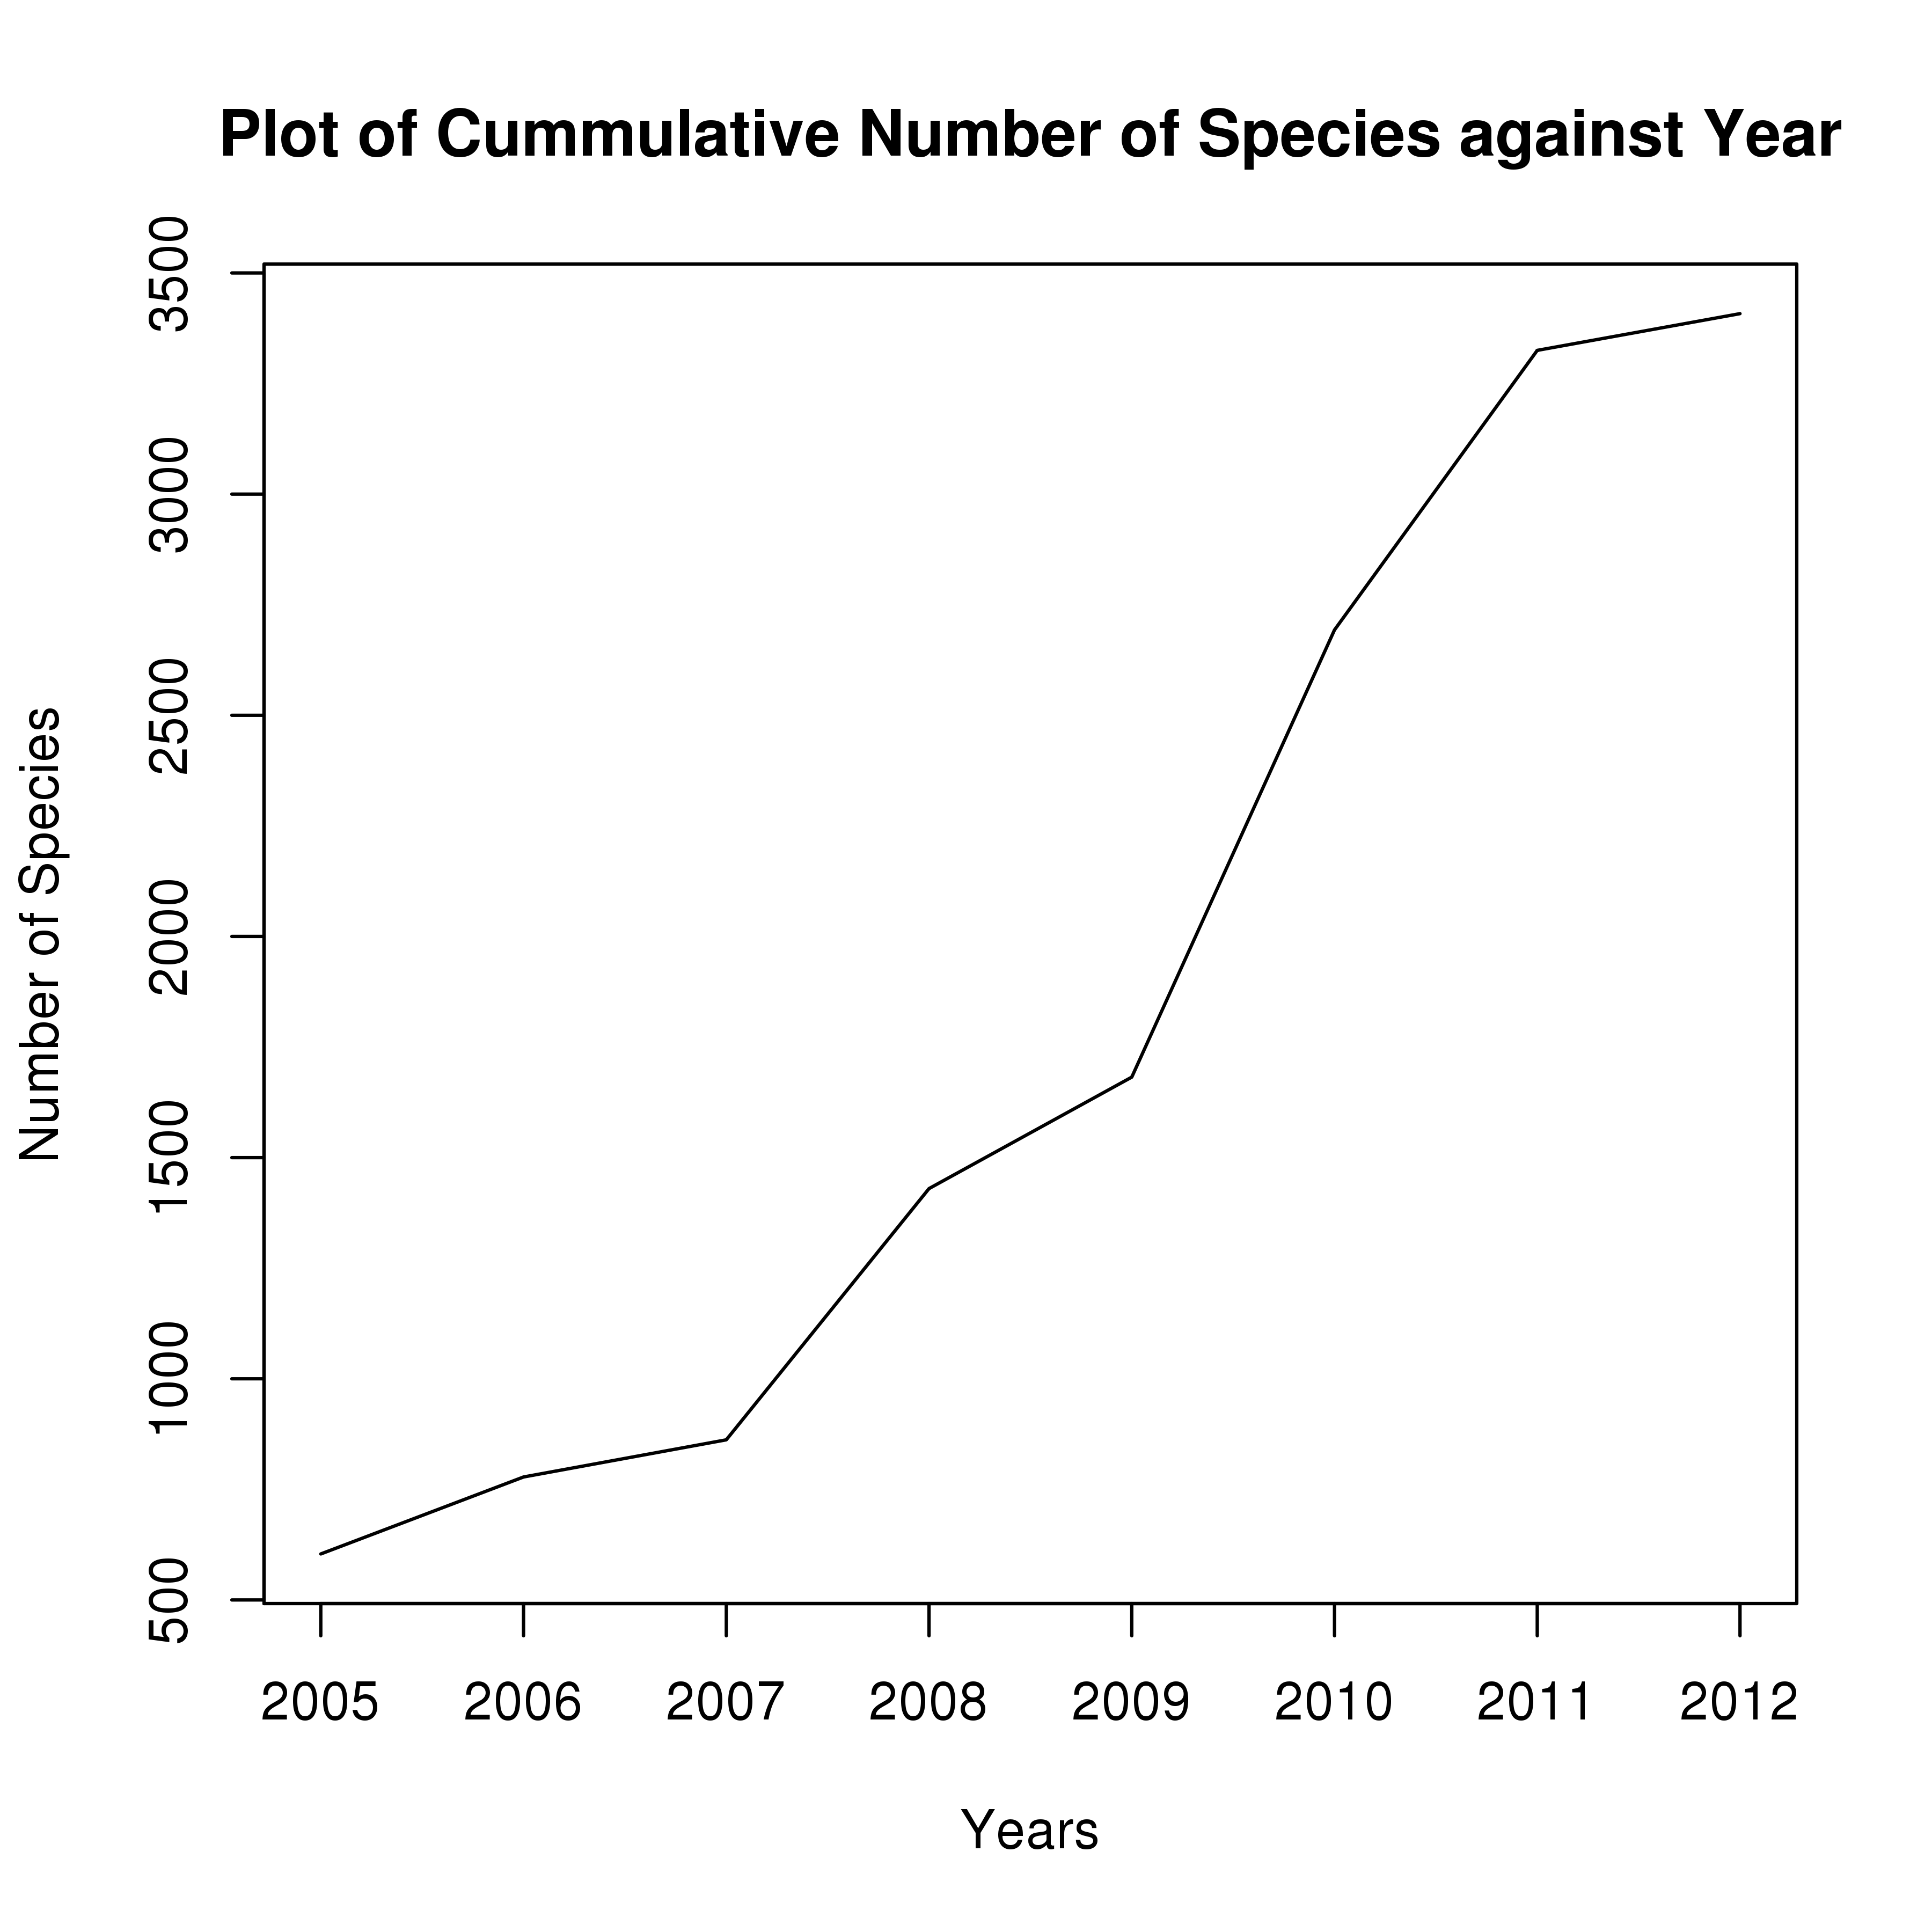
\includegraphics[trim= 1.5mm 5mm 5mm 4.5mm, clip, scale=0.4]{Poster-images/CummulativeSpeciesPlot.png}
 The graph above shows the number of species in the curated branch against time. There is no clear pattern to how the number of species increases over time, except that a large increase in one year precedes a smaller increase in the next year.
 
 Since there has been a smaller increase in the total number of models in 2012, the small increase in the total number of species in 2012 is expected.
 \end{multicols}
 }
 
 \headerbox{SBML}{name=sbml,column=0,span=2,below=r}{
 Systems Biology Markup Language (SBML) is a modelling standard used for exchanging models between different software tools. An example of some SBML code is shown below. This code definines the species for one of the biomodels:
 
 \begin{flushleft}
 {\scriptsize{
  \color{blue}
 <\color{red}listOfSpecies\color{blue}>
 
 <\color{red}species metaid$\color{blue}=$\color{blue}"$\color{black}\_230475$\color{blue}" \color{red} id$\color{blue}=$\color{blue}"\color{black}C\color{blue}" \color{red} name$\color{blue}=$\color{blue}"\color{black}Cyclin\color{blue}" \color{red} compartment$\color{blue}=$\color{blue}"\color{black}cell\color{blue}" \color{red} initialConcentration$\color{blue}=$\color{blue}"$\color{black}0.01$\color{blue}" \color{red} substanceUnits$\color{blue}=$\color{blue}"\color{black}substance\color{blue}" \color{red} sboTerm$\color{blue}=$\color{blue}"\color{black}SBO:$0000252$\color{blue}"/>
 
 <\color{red}species metaid$\color{blue}=$\color{blue}"$\color{black}\_230495$\color{blue}" \color{red} id$\color{blue}=$\color{blue}"\color{black}M\color{blue}" \color{red} name$\color{blue}=$\color{blue}"\color{black}CDC-2 Kinase\color{blue}" \color{red} compartment$\color{blue}=$\color{blue}"\color{black}cell\color{blue}" \color{red} initialConcentration$\color{blue}=$\color{blue}"$\color{black}0.01$\color{blue}" \color{red} substanceUnits$\color{blue}=$\color{blue}"\color{black}substance\color{blue}" \color{red} sboTerm$\color{blue}=$\color{blue}"\color{black}SBO:$0000252$\color{blue}"/>
 
 <\color{red}species metaid$\color{blue}=$\color{blue}"$\color{black}\_230515$\color{blue}" \color{red} id$\color{blue}=$\color{blue}"\color{black}X\color{blue}" \color{red} name$ \color{blue}=$ \color{blue} "\color{black}Cyclin Protease\color{blue}" \color{red} compartment$\color{blue}=$\color{blue}"\color{black}cell\color{blue}" \color{red} initialConcentration$\color{blue}=$\color{blue}"$\color{black} 0.01$\color{blue}" \color{red} substanceUnits$\color{blue}=$\color{blue}"\color{black}substance \color{blue}" \color{red} sboTerm$\color{blue}=$\color{blue}"\color{black}SBO:$0000297$\color{blue}"/>
 
 <\color{red}/listOfSpecies color{blue}>}}
 \end{flushleft}
 
 Since every process in a biological cell can be broken down into one or more chemical transformations, SBML represents models as a list of these transformations. 
 
 Whilst SBML is easy for computers to generate and parse, it is difficult for humans to read and write. In order to extract information from the models, the SBML files for the models were first read into R and transformed into objects that can be worked with in R.
 }
 
 \headerbox{Terms}{name=terms,column=0,span=2,below=sbml}{
 \begin{multicols}{2}
 Consider we have a chemical called X. Let there be a model which describes how the amount of X varies with time. Finally, let the rate of change of the amount of X be described by the following equation:\\
 
 $\frac{dX(t)}{dt} = k_1 X(t) + k_2$\\
 
 Where the amount of X is altered by the following processes:\\
 
 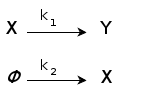
\includegraphics[scale=0.4]{Poster-images/TermDiagram.png}
 
 \begin{itemize}
 \item The entities X, Y and Z are species. Species range from chemicals such as ions or molecules to biological entities such as protein binding sites.
  
 \item The process altering the amount of X are reactions. Reactions are the processes by which the amounts of the species in a model change. The most common type involves a set of chemicals (reractants) being transfromed to another set of chemcials (products).
 
 \item $k_1$ and $k_2$ are parameters. Parameters are the numbers used in the desrciption of the rate laws of reactions, these rate laws describe how a species varies over time.
 
 \end{itemize}
 \end{multicols}
 }
 
  \headerbox{Connections}{name=connections,column=0,below=terms}{
 In this project, a species is defined as having a 'connection' in a particular reaction if the sepcies occurs in that reaction.\\
 
 Consider the following set of reactions:
 
 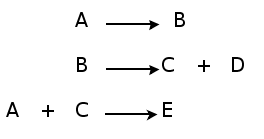
\includegraphics[scale=0.4]{Poster-images/connectiondrawing.png}
 
 Since the species A, B and C each appear in 2 reactions in the set, they each have 2 connections in this set. The species D and E appear in just 1 reaction and so have just 1 connection in this set.
 
 The average number of connections per species in the database is 5.334 (to 3 decimal places). 
 }
 
 \headerbox{SBO Terms}{name=sboterms,column=1,below=terms}{
 SBO is an acronym for Systems Biology Ontology. Its main use is in the field of systems biology. SBO terms help to provide additional information to the modeller, such as showing the role participants have in certain reactions. 

In the project, the possibility of using SBO terms to track which models certain species apperared in was explored. The table below shows the frequency of the SBO terms for the species in the first model:

  \begin{flushleft}
    {\footnotesize{
    \begin{tabular}{ | p{1.7cm} | p{2.29cm} | p{1.2cm} | }
    \hline
    sboTerm & Model ID & Frequency \\ \hline
    SBO:0000297 & $\text{\textnormal{EPSP\_Edelstein}}$ & 8 \\ \hline
    SBO:0000420 & $\text{\textnormal{EPSP\_Edelstein}}$ & 4 \\
    \hline
    \end{tabular}}}
  \end{flushleft}
  
  As shown above, since there are multiple species with the same SBO term, it is not posssible to use the SBO terms to find in which model a particular species is present.
}
 
 \headerbox{Parameters}{name=paras,column=2,span=2,below=specsnreacts}{
 \begin{multicols}{2}
 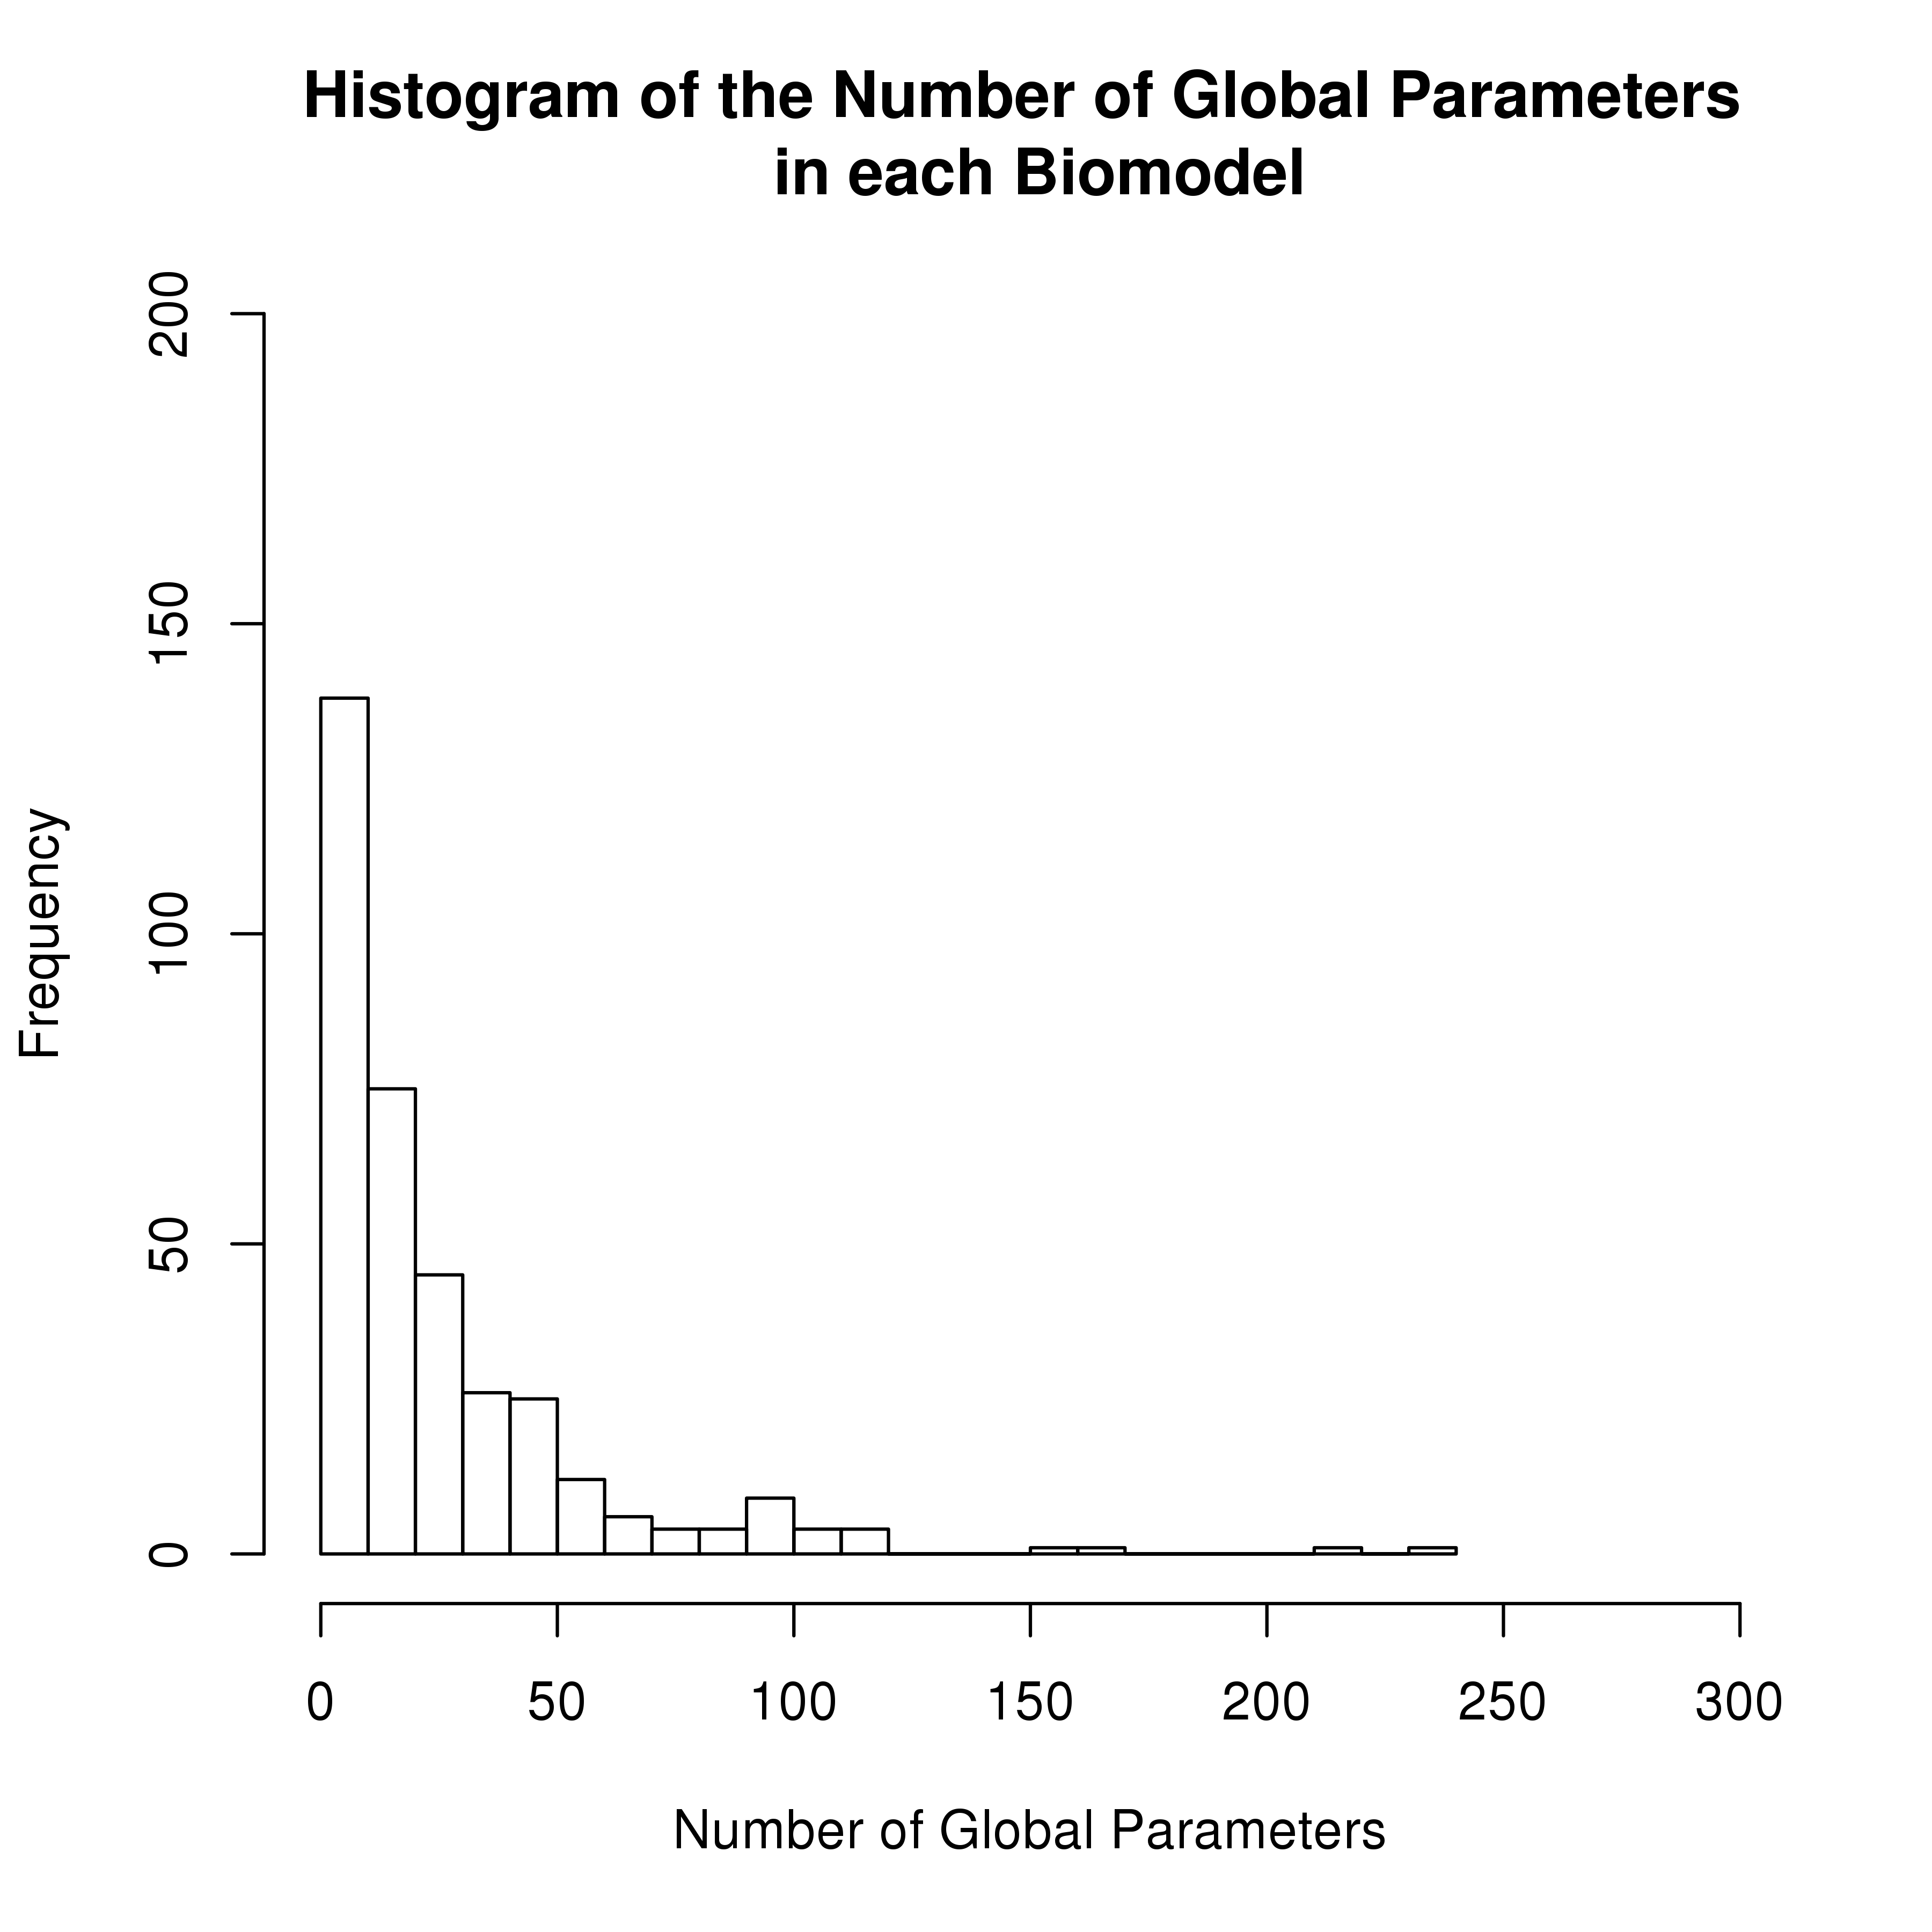
\includegraphics[trim= 1.5mm 5mm 5mm 5mm, clip, scale=0.4]{Poster-images/GlobalParametersHistogram.png}
  The graph above shows the number of global parameters in each biomodel. The majority of models have 20 or less global parameters, with over 100 having less than 10 global parameters. This suggests that the models tend to have a low number of global parameters.

 
 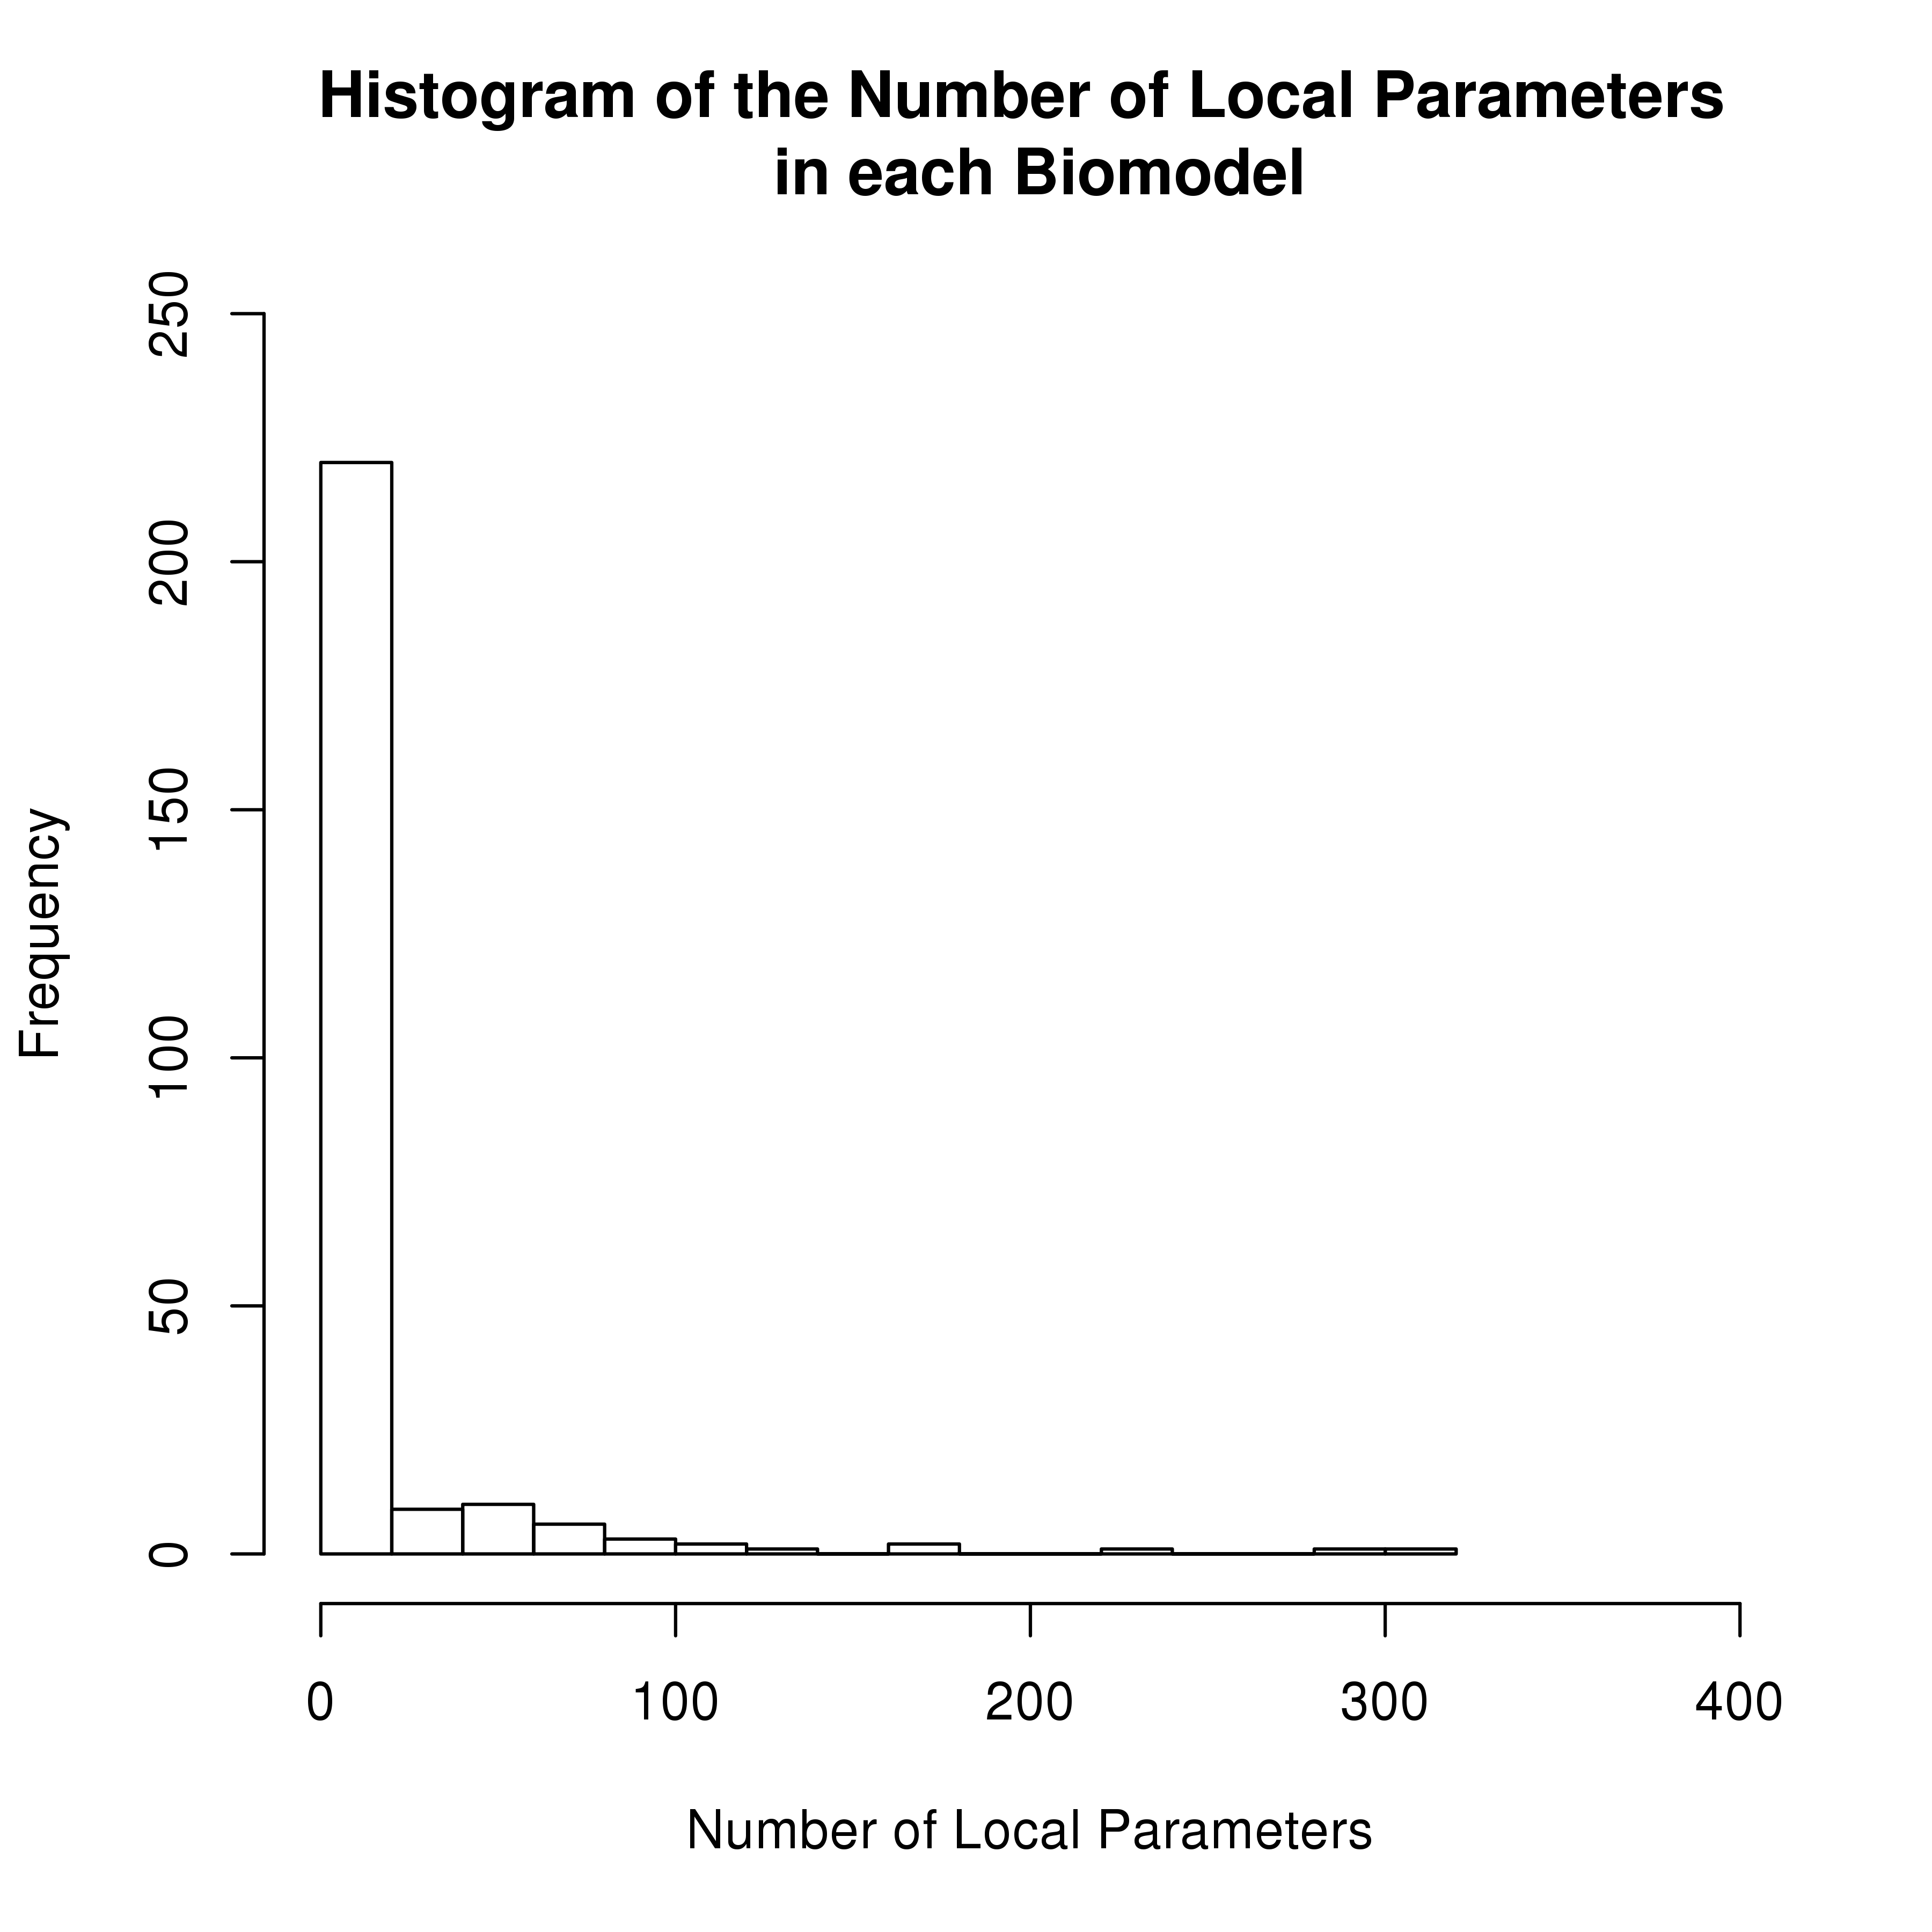
\includegraphics[trim= 1.5mm 5mm 5mm 5mm, clip, scale=0.4]{Poster-images/LocalParametersHistogram.png} 
 The graph above shows the number of local parameters in each biomodel. The majority of models have 10 or less local parameters, due to a large proportion 0f models defining all their parameters as global parameters. This suggests that the models tend to have a low number of local parameters.
 \end{multicols}
 }
 
\end{poster}

\end{document}